\singlespacing

\begin{figure}[h]
	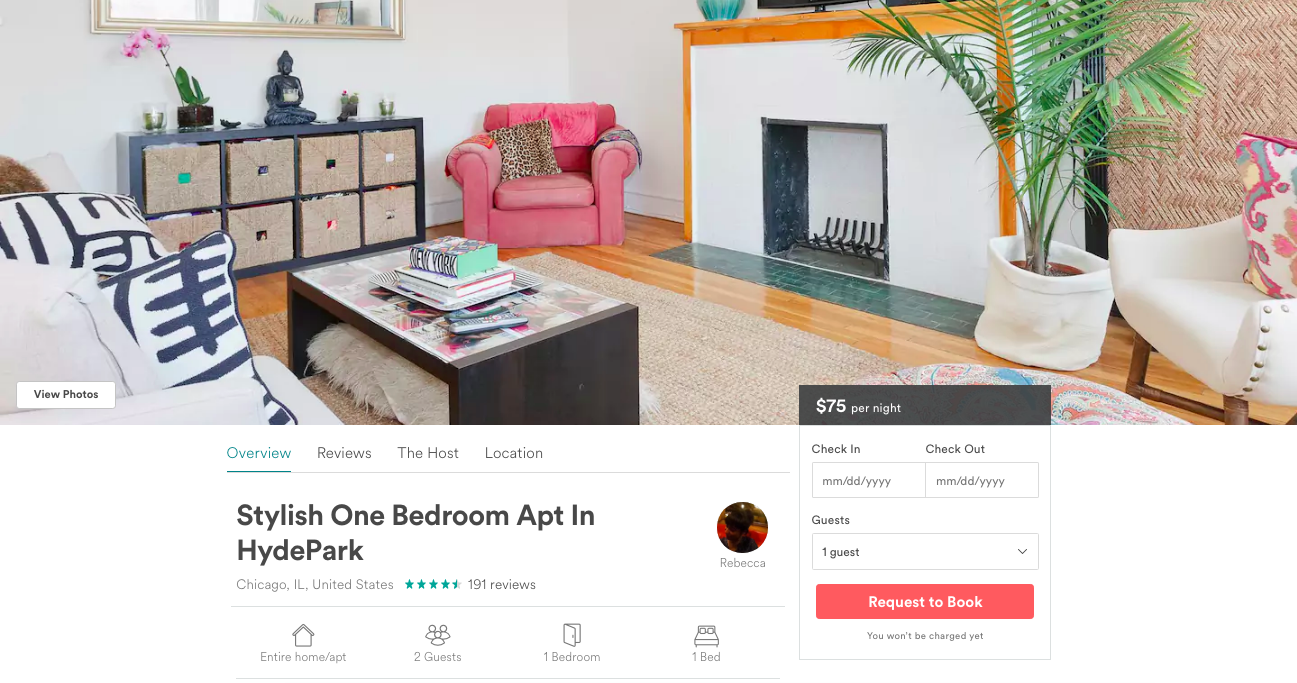
\includegraphics[width=1\textwidth]{tables/sample1-cover}
	\caption{Sample listing profile from Chicago}
	\label{fig:listing}
\end{figure}
\begin{figure}
	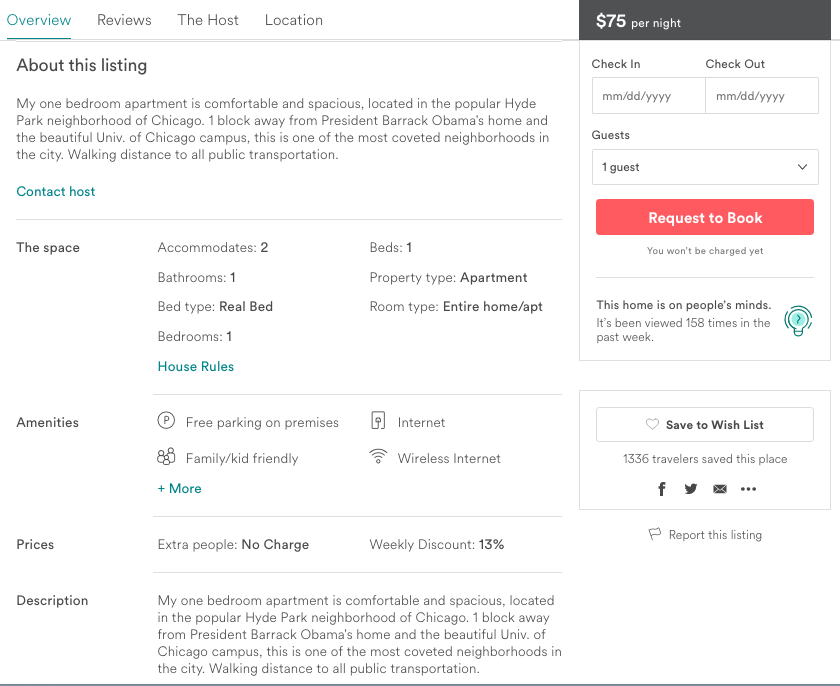
\includegraphics[width=1\textwidth]{tables/sample2-property}
	\caption{Sample property characteristics}
	\label{fig:property}
\end{figure}

%Histograms
\begin{figure}\centering
	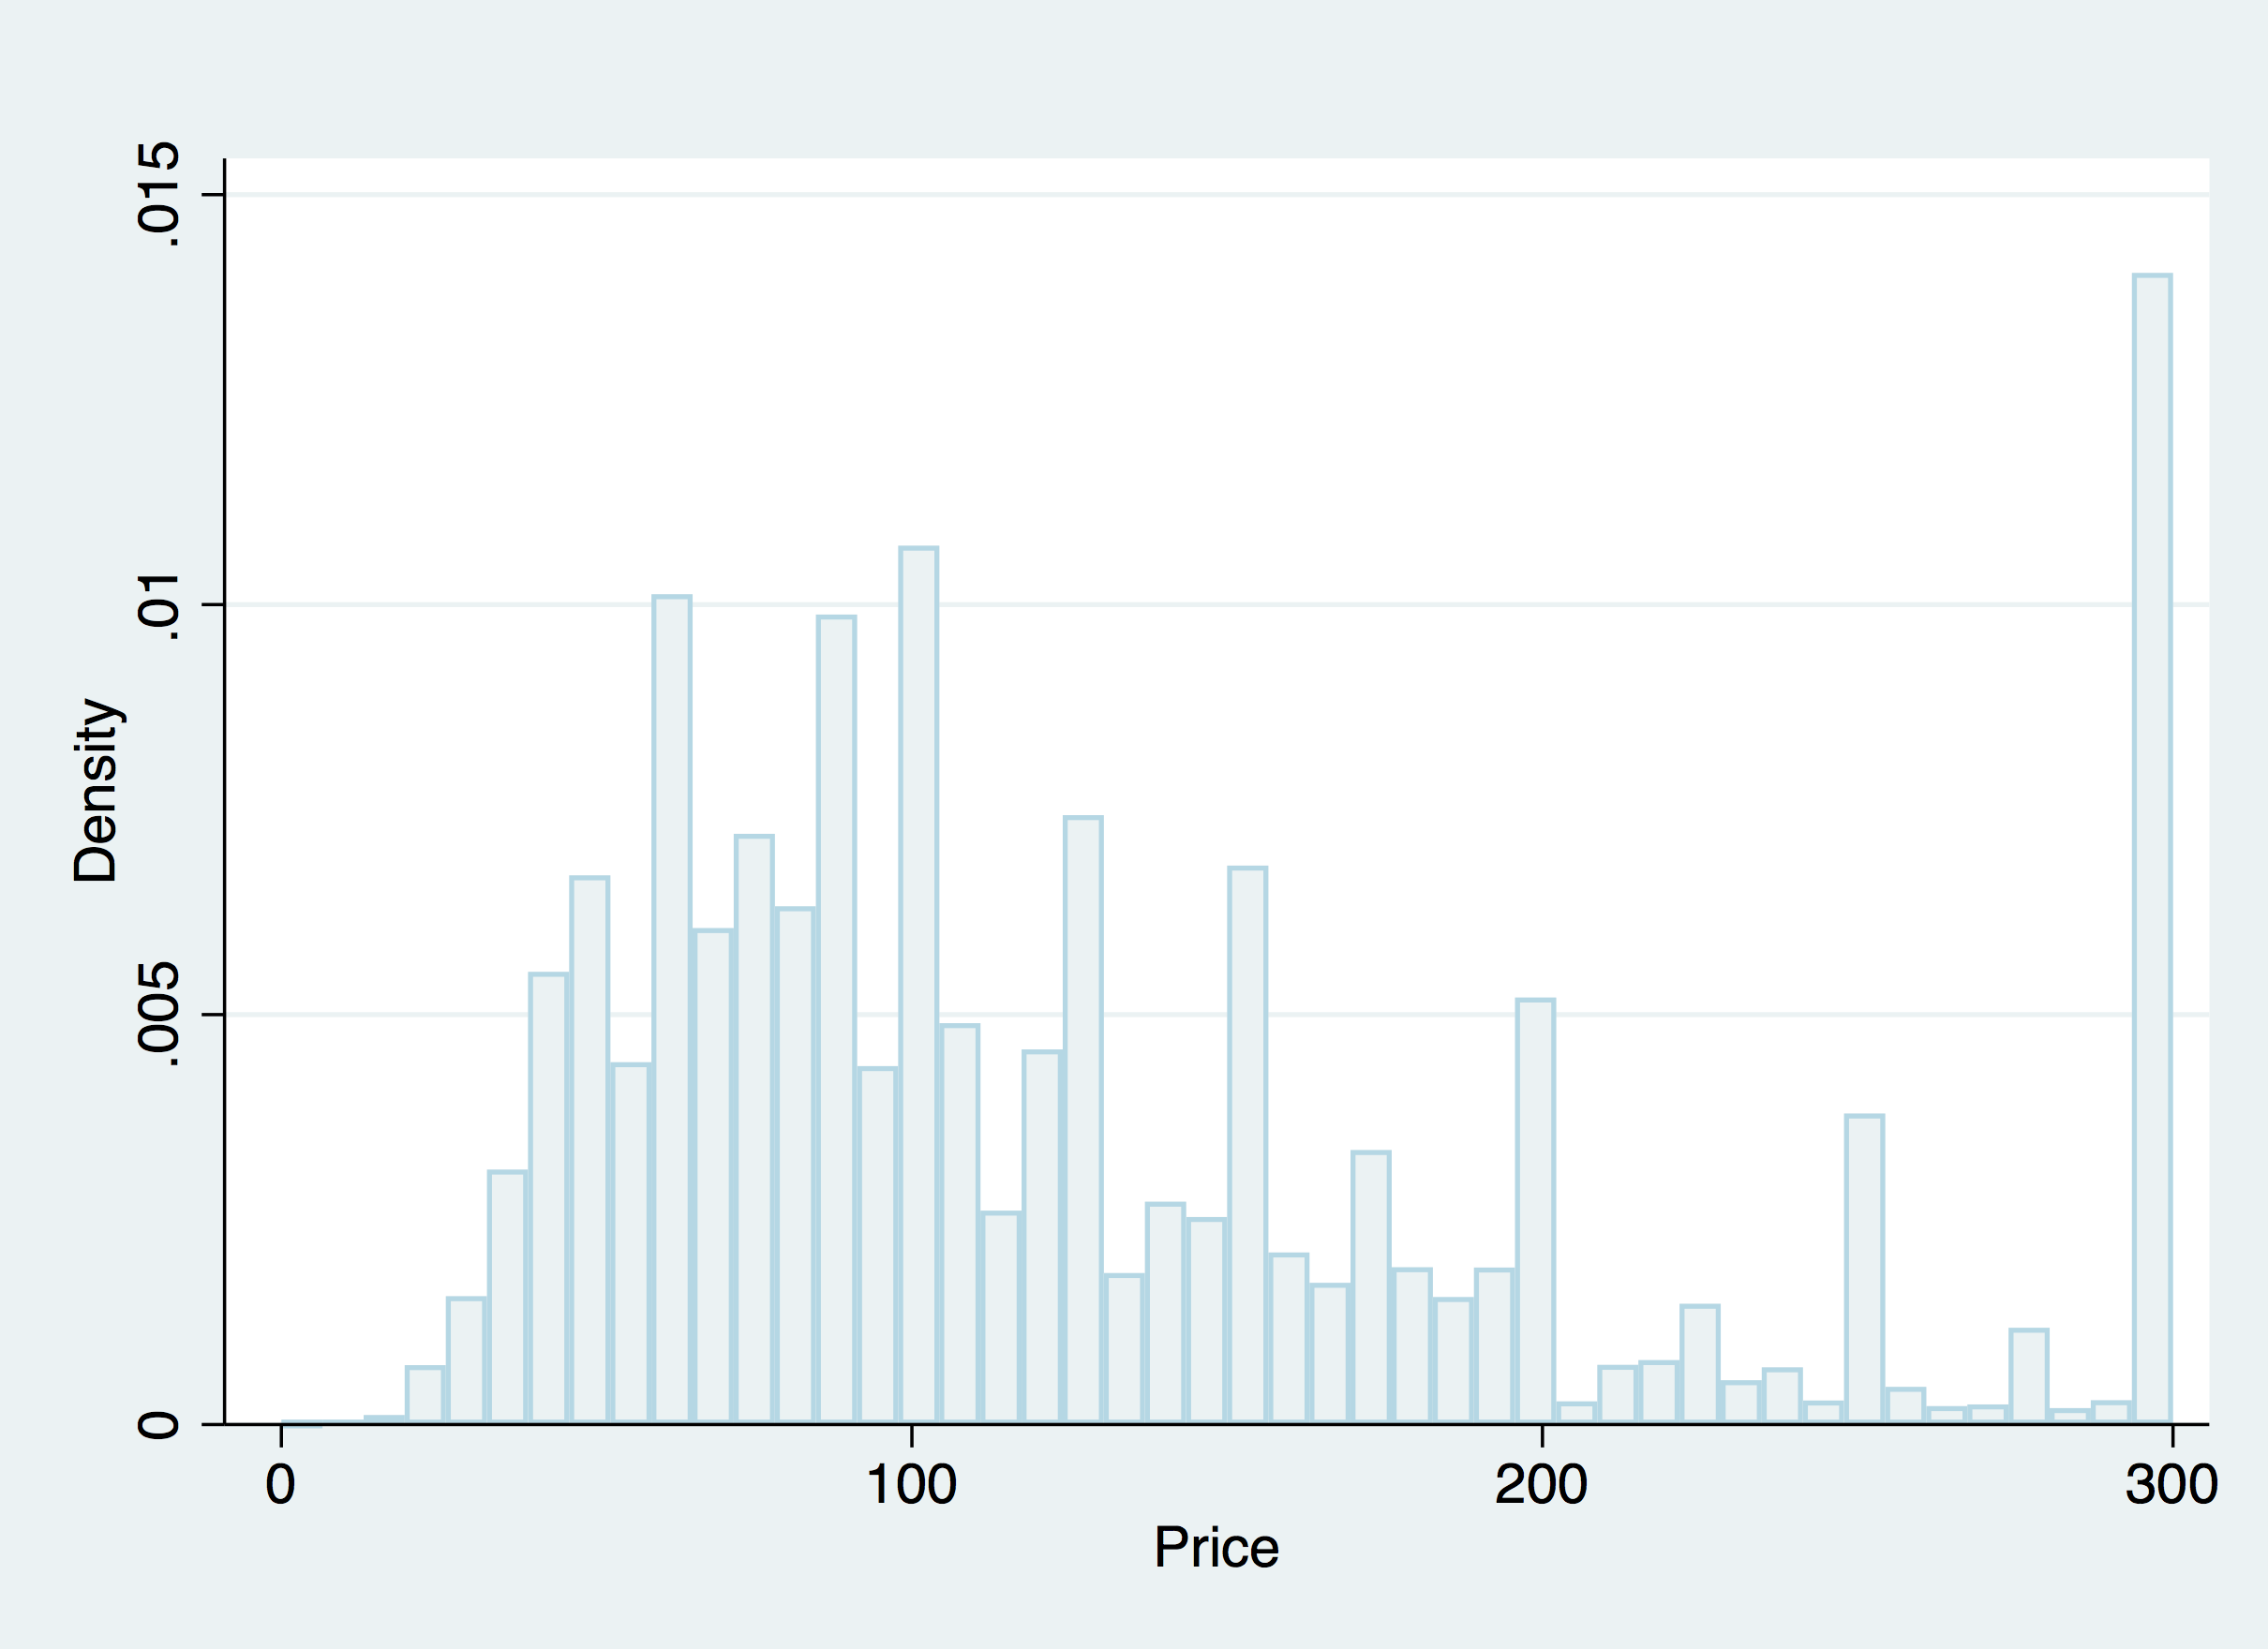
\includegraphics[width=.8\textwidth]{figures/price_dist-CONT-300}
	\caption{Distribution of prices}
	\caption*{Notes: All the listings priced at \$300 or more are grouped together at price = 300}
	\label{fig:prices}
\end{figure}

\begin{figure}\centering
	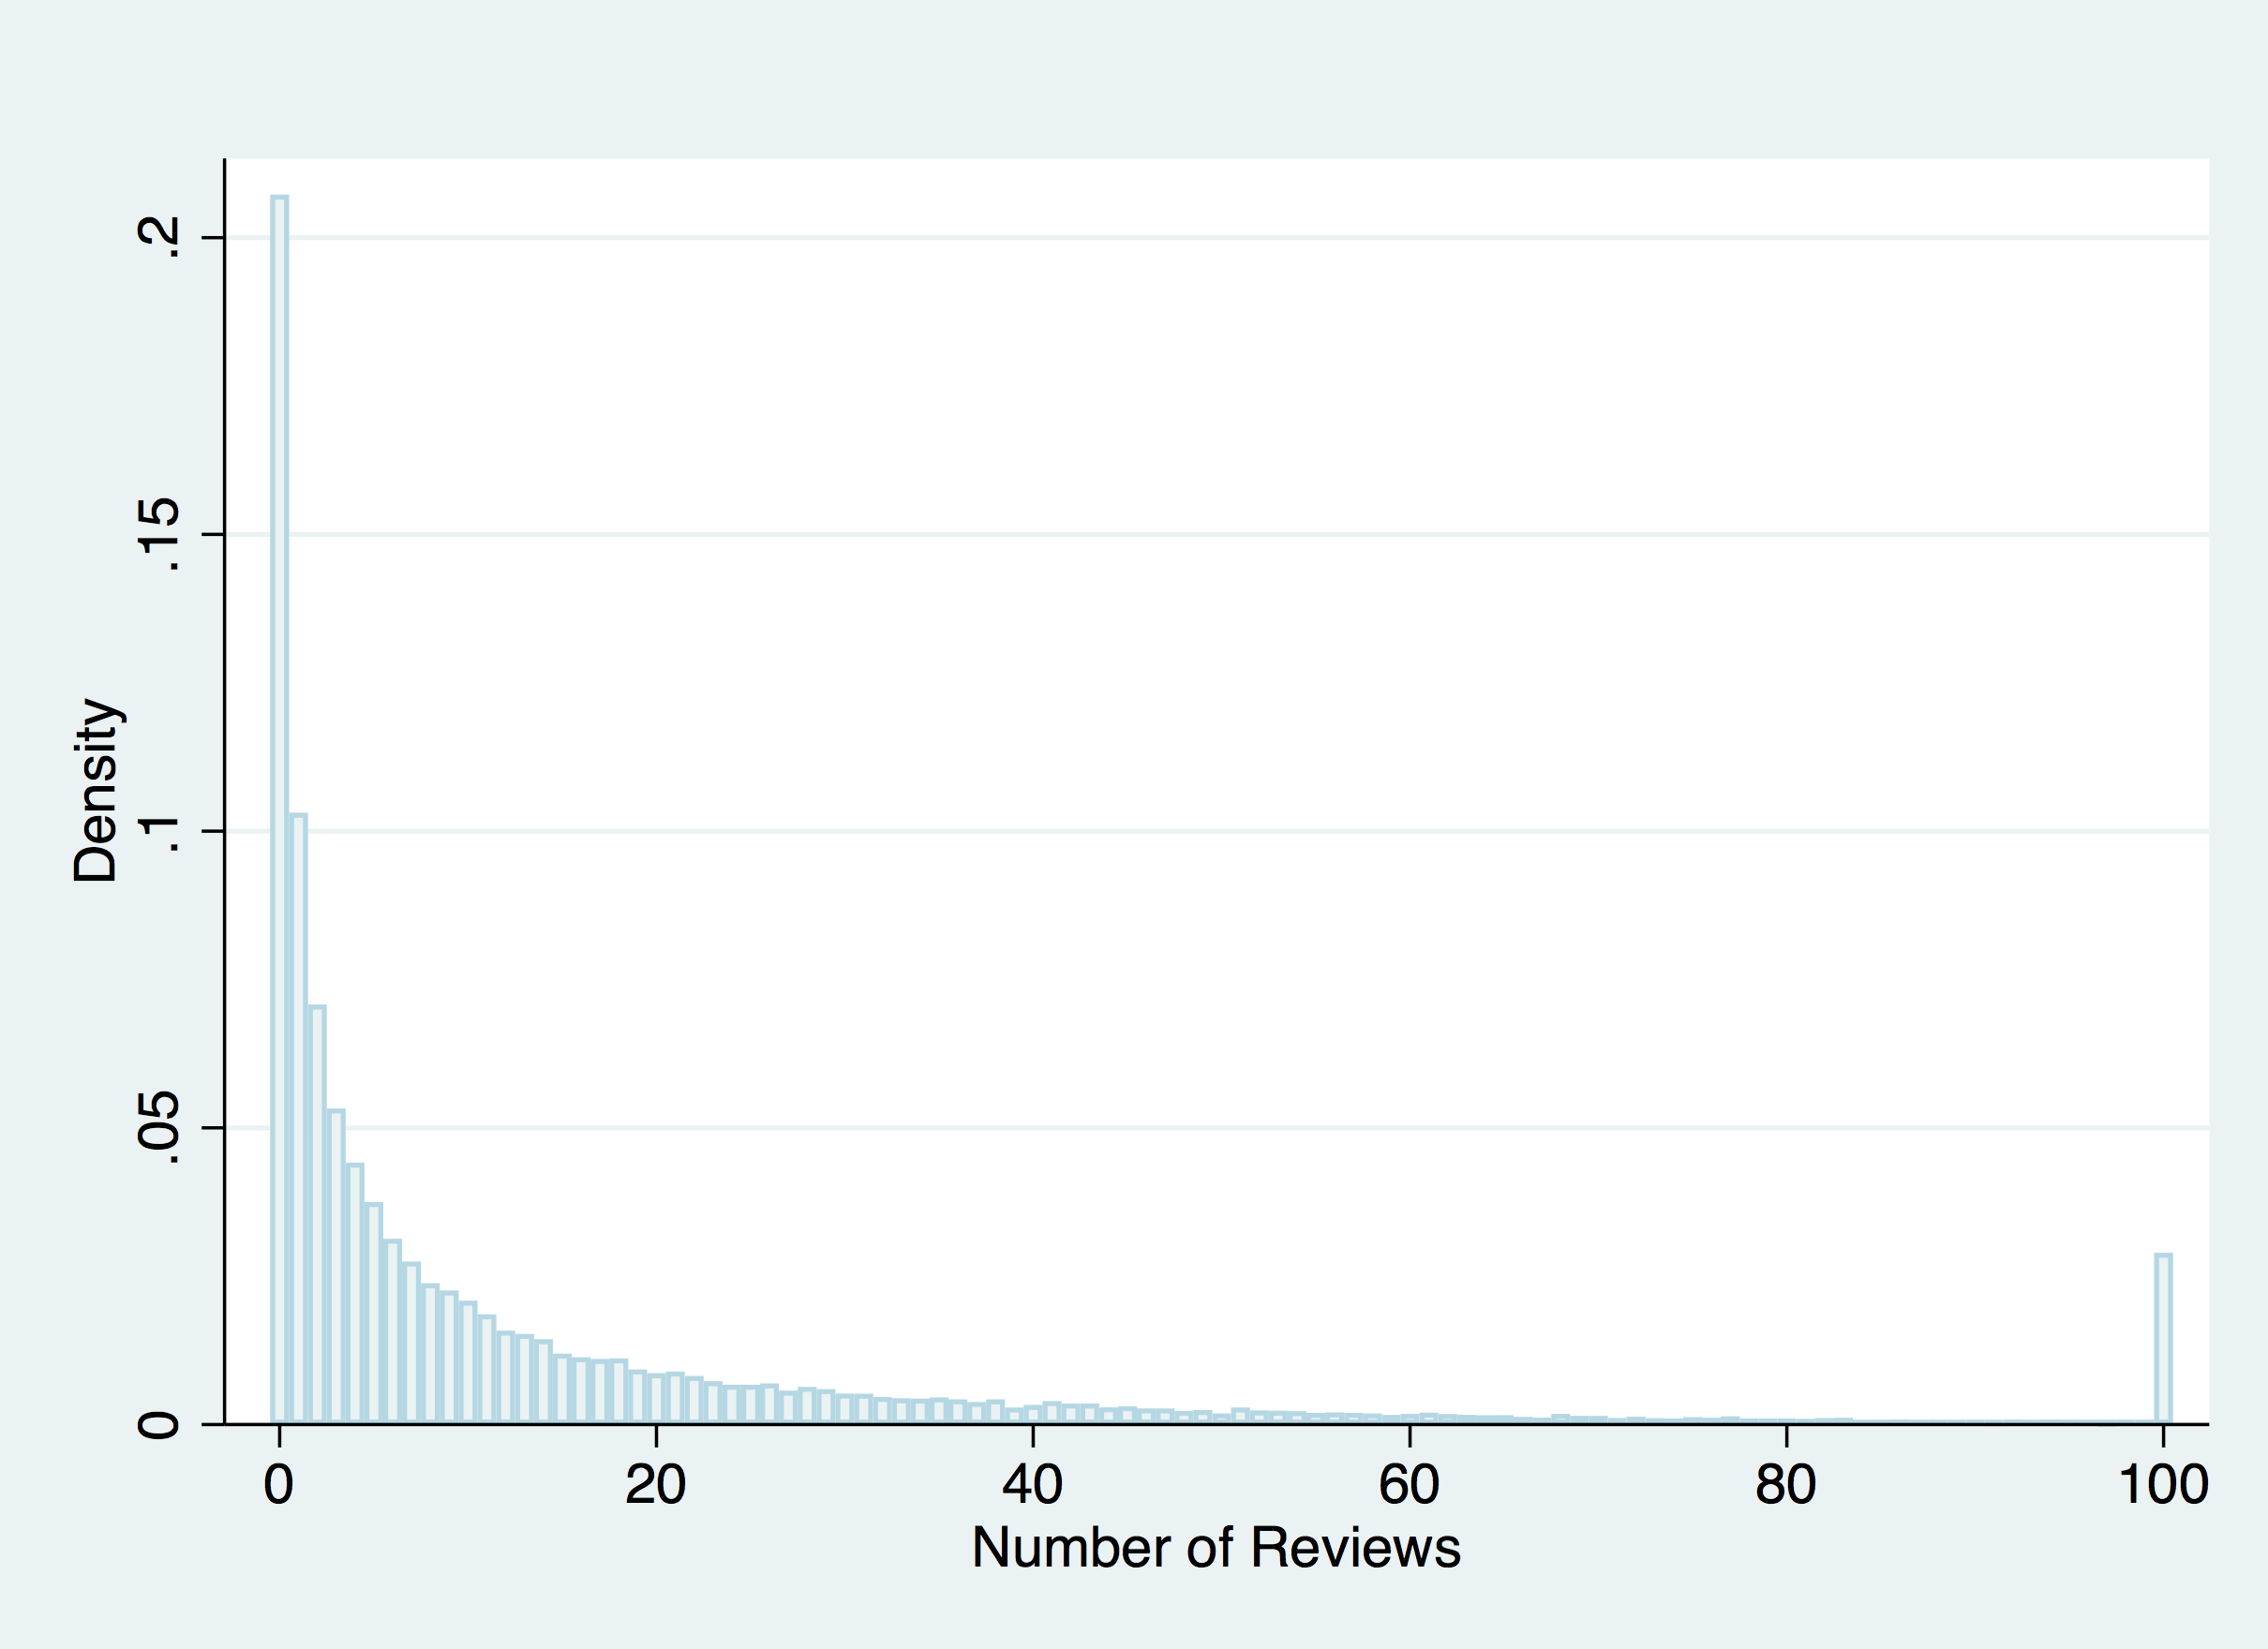
\includegraphics[width=.8\textwidth]{figures/num_reviews_dist-DISC-100}
	\caption{Distribution of number of reviews}
	\caption*{Notes: All the listings with 100 reviews or more are grouped together at number of reviews = 100}
	\label{fig:reviews}
\end{figure}

\begin{figure}\centering
	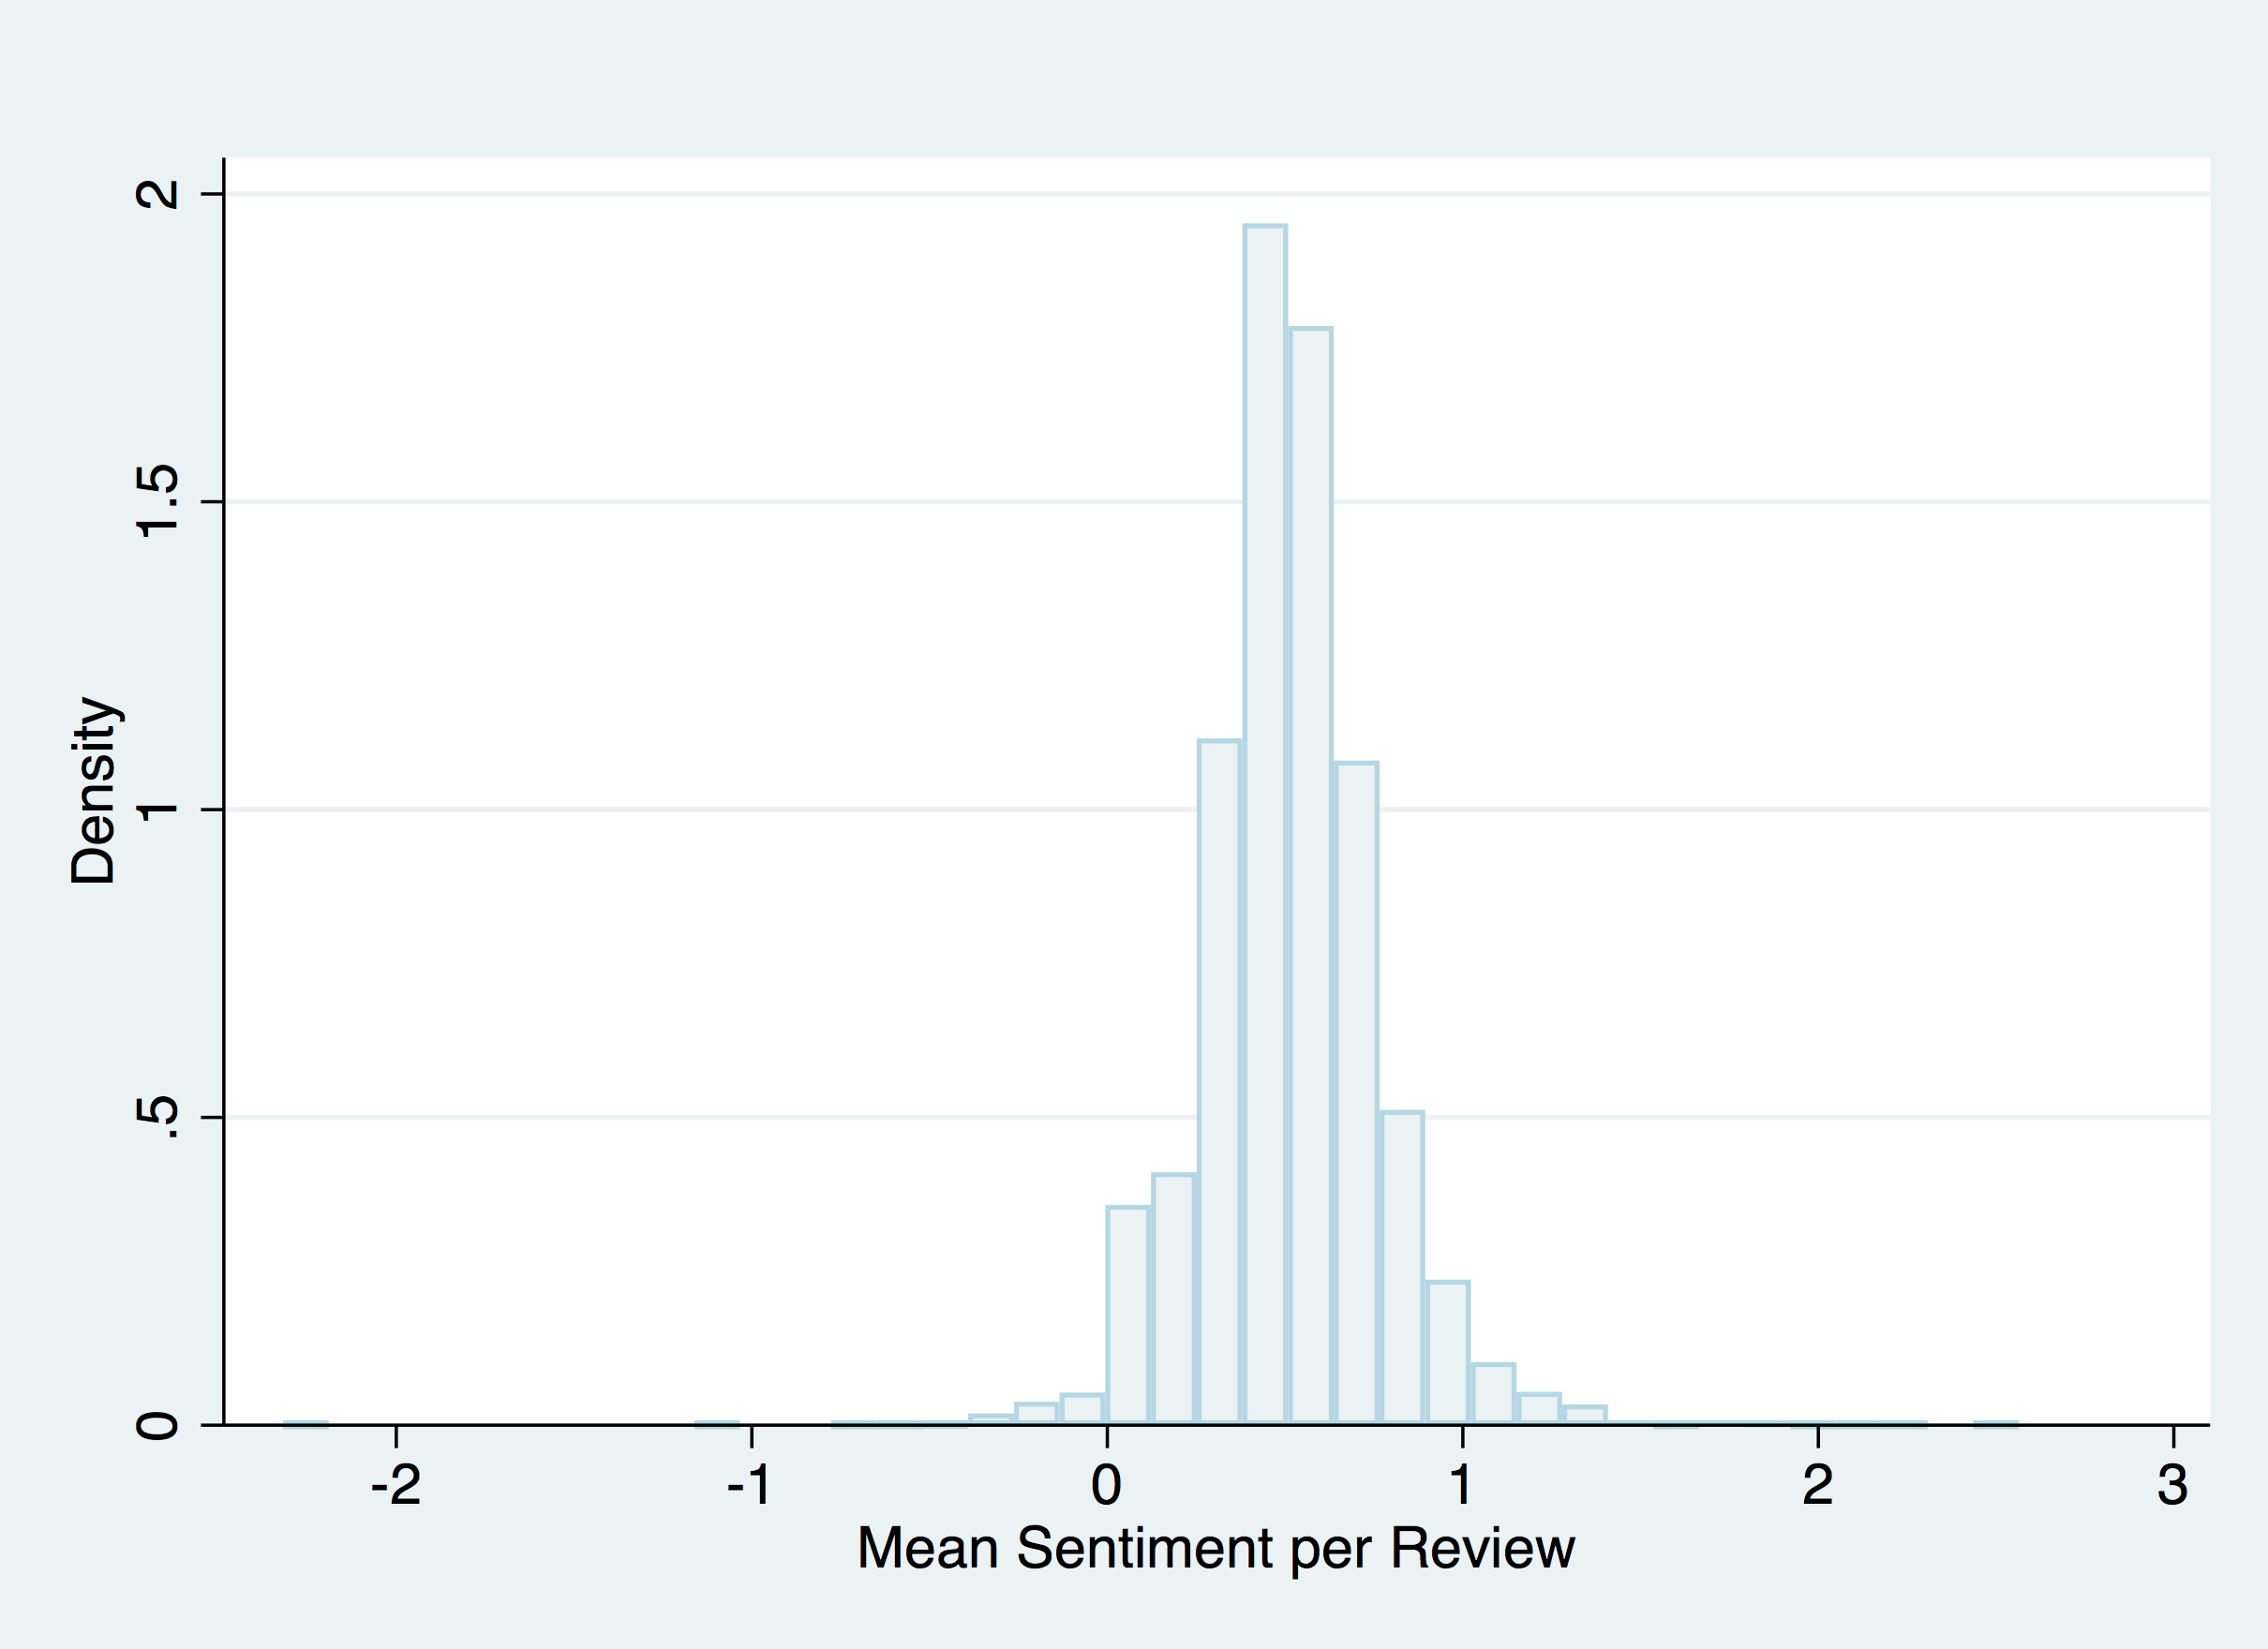
\includegraphics[width=.8\textwidth]{figures/review_sentiment_dist}
	\caption{Distribution of review sentiment}
	\label{fig:sentiment}
\end{figure}


%1
%listing-level summary table
\small
{
\begin{longtable}{l*{6}{c|c|cccc}}
	\caption{Summary Statistics by Host Race: Listing Characteristics}\\
	\hline
     &\multicolumn{1}{c}{Full data}&\multicolumn{1}{c}{}&\multicolumn{1}{c}{}&\multicolumn{1}{c}{Regression sample}&\multicolumn{1}{c}{}&\multicolumn{1}{c}{}\\
      \cline{3-7}\\
     &\multicolumn{1}{c}{}&\multicolumn{1}{c}{All}&\multicolumn{1}{c}{White}&\multicolumn{1}{c}{Black}&\multicolumn{1}{c}{Hispanic}&\multicolumn{1}{c}{Asian}\\
     \hline\hline
             
\textit{Outcome variables} \\
Price (\$/day)        & 175.72  &     167.37         &      178.62      &     125.95      &     160.39       &   131.06\\
                  & (294.14) &         (277.7)         &         (289.4)         &         (208.1)         &         (275.0)     & (242.1)    \\
Number of reviews     & 17.51  &      16.57  &      17.14         &      15.06&      16.46 & 	14.08\\
                 & (31.86)  &     (30.8)         &     (31.9)         &     (27.2)         &     (29.7)        & (27.6) \\
                 
\textit{Covariates} \\
\hline
Property Type \\
\hspace{3mm} Apartments/Lofts     		&	.577 &      .598         &       .590         &      .654        &      .625 			& 	.601         \\
\hspace{3mm} Townhouses/Condos   &  .042 &      .042         &      .039         &      .041        &      .041 	& 		.055         \\
\hspace{3mm} Houses    				&.321	&      .321         &       .336        &      .279        &      .289				& 		.311         \\
\hspace{3mm} Other    				&.06	&      .039      &       .035        &      .026        &      .045	& 		.033        \\

Room Type \\
\hspace{3mm} Entire home/apt   &  .577 & .577   	&      .607	&      .449  &      .510		&    .418\\
\hspace{3mm} Private room       & .384 & 	.384		&      .363	&      .483  &      .434		&    .530\\
\hspace{3mm} Shared room      & .039 &	.04	 	&      .029	&      .067  &      .056		&    .052\\

Max Num. Guests   & 3.44   &      3.26	&      3.36  &      2.90		&    3.17 		&	 2.89\\
               & (2.41)    &     (2.3)         &     (2.3)         &     (2.1)         &     (2.4)         & (2.1)\\
Bedrooms    &  1.35 &      1.30 &      1.33         &      1.20         &      1.25   & 1.20      \\
              &   (.92)   &     (.88)         &     (.92)         &     (.72)         &     (.90)       & (.76)  \\
Bathrooms  & 1.30  &      1.27         &       1.29         &      1.20         &      1.26 & 1.21         \\
                &  (.69)  &     (.66)         &     (.68)         &     (.52)         &     (.69)         & (.58)\\
Beds       & 1.82  &      1.73 &      1.76         &      1.63         &      1.74         & 1.59\\
               &   (1.41)  &     (1.32)         &     (1.31)         &     (1.22)         &     (1.60)   & (1.21)      \\
Availability (out of 30 days)    & 11.53   &      11.30&      10.9&      14.4 &      11.46  	& 	10.88\\
         &  (10.93)    & (10.99)     &     (10.85)  &     (11.54)  &     (11.03)         &     (11.05)         \\
Number of Amenities   &   .81  &      .80		&      .81&      .77 &      .80  	& 	.75\\
         						  &  (1.10)  & (1.10)     &     (1.11)    &     (1.05)         &     (1.10)         &     (1.13)         \\
Cleaning Fee   &  67.94 &      FIX	&      .81&      .77 &      .80  	& 	.75\\
						&  (60.36)  & (FIX)     &     (1.11)         &     (1.05)         &     (1.10)     &     (1.13)         \\
Extra Guests Charge   &   13.74  &  FIX      &    .81  &      .77           &   .80  	& 	.75\\
									&  (23.65)  & (1.10)  &     (1.11) &     (1.05)     &     (1.10) &     (1.13)  \\
Instantly Bookable?   &   .15  &      FIX		&      .81&      .77 &      .80  	& 	.75\\
									&  (.361)  & (1.10)     &     (1.11)  &     (1.05)   &     (1.10)   &     (1.13)         \\
Minimum Nights   &   3.01  &      FIX		&      .81&      .77 &      .80  	& 	.75\\
							&  (9.21)  & (1.10)     &     (1.11)         &     (1.05)         &     (1.10)         &     (1.13)         \\
Strict Cancellation Policy   &   .43  &      FIX		&      .81&      .77 &      .80  	& 	.75\\
[1em]
Year of first review    & 14.86   &      FIX	&      3.36  &      2.90		&    3.17 		&	 2.89\\
							& (1.22)    &     (FIX)         &     (2.3)         &     (2.1)         &     (2.4)         & (2.1)\\

\hline
Observations  & 69,007  & 68,983   &       43,988         &       5,023         &       3,524   & 5,893      \\
\hline\hline
\caption*{Notes: The values in the table are means and standard deviations of listing-level data in my full sample. Summary statistics for selected covariates are listed in the table. Categorical variables such as room type do not have standard deviations. Property types are explicitly listed if more than 1.5\% of listings are that type. Only the most popular cancellation policy type is listed - in the full sample, 99\% of listings have strict (43\%), flexible (31\%) or moderate (25\%) cancellation policies. Year of first review is a proxy for the time on the market - 14.86 indicates that the first review of the mean listing in the full sample occured in October of 2014.}

\end{longtable}
}
\normalsize




% \include{code/output/ }

%2
%Host-level summary table
{
	\def\sym#1{\ifmmode^{#1}\else\(^{#1}\)\fi}
	\begin{longtable}{l*{6}{c}}
		\caption{Summary Statistics by Race: Host Demographics}\\
		
		\hline
		&\multicolumn{1}{c}{}&\multicolumn{1}{c}{}&\multicolumn{1}{c}{}&\multicolumn{1}{c}{Regression}&\multicolumn{1}{c}{}&\multicolumn{1}{c}{}\\
		\cline{3-7}\\
			&\multicolumn{1}{c}{Full data}&\multicolumn{1}{c}{Full Sample}&\multicolumn{1}{c}{White}&\multicolumn{1}{c}{Black}&\multicolumn{1}{c}{Hispanic}&\multicolumn{1}{c}{Asian}\\
		
		\hline\hline\endfirsthead\hline\endhead\hline\endfoot\endlastfoot
		&\multicolumn{1}{c}{(1)}&\multicolumn{1}{c}{(2)}&\multicolumn{1}{c}{(3)}&\multicolumn{1}{c}{(4)}&\multicolumn{1}{c}{(5)}&\multicolumn{1}{c}{(6)}\\
		&\multicolumn{1}{c}{Full data}&\multicolumn{1}{c}{Regression sample}&\multicolumn{1}{c}{White}&\multicolumn{1}{c}{Black}&\multicolumn{1}{c}{Hispanic}&\multicolumn{1}{c}{Asian}\\
		\hline
		\endhead             
		     
		\textit{Host demographics} \\
		\hline
		\textit{Race} \\
		White     & &      .637         &       1.00         &      0         &      0 	& 		0         \\
		Black     &  &    .073       &       0         &      1.00         &      0 	& 		0         \\
		Hispanic     & &      .051         &       0         &      0         &      1.00 	& 		0         \\
		Asian     &   &   .085      &       0         &      0         &      0 	& 		1.00         \\
		Unknown/Multiracial     & &      .152         &       0         &      0         &      0 	& 		0         \\
		[1em]
		\textit{Sex} \\
		Male     & &      .309         &       .356         &      .354         &      .417 	& 		.367        \\
		Female     & &      .378         &       .427        &      .541         &      .426 	& 		.476         \\
		Unknown/Two people   &  &      .312         &       .216         &      .104         &      .156 	& 		.157         \\
		[1em]
		\textit{Age} \\
		Young ($<$ 30)     & &      .427         &       .469         &      .514        &      .481 	& 		.587         \\
		Middle-aged     & &      .421         &       .491        &      .470         &      .490 		& 		.379         \\
		Old ($>$ 65)     & &      .018         &       .026         &      .004         &      .009	& 		.009         \\
		Unknown    &  &      .133         &       .013         &      .011         &      .018 	& 		.024         \\
		[1em]

		
		\hline
		Observations (full sample)    &  & 68,983   &       43,988         &       5,023         &       3,524         &       5,893         \\
		\hline\hline
		\caption*{Notes: The values in the table are means and standard deviations of host-level data in my full sample. Summary statistics for selected covariates are listed in the table. Categorical variables such as race, sex, and age do not have standard deviations. White refers only to Non-Hispanic Whites.}
		
	\end{longtable}
}



%3
%Host-level summary table
{
	\def\sym#1{\ifmmode^{#1}\else\(^{#1}\)\fi}
	\begin{longtable}{l*{6}{c}}
		\caption{Summary Statistics by Race: Host Characteristics}\\
		
		\hline
		&\multicolumn{1}{c}{}&\multicolumn{1}{c}{}&\multicolumn{1}{c}{}&\multicolumn{1}{c}{Regression}&\multicolumn{1}{c}{}&\multicolumn{1}{c}{}\\
		\cline{3-7}\\
			&\multicolumn{1}{c}{Full data}&\multicolumn{1}{c}{Full Sample}&\multicolumn{1}{c}{White}&\multicolumn{1}{c}{Black}&\multicolumn{1}{c}{Hispanic}&\multicolumn{1}{c}{Asian}\\
		
		\hline\hline\endfirsthead\hline\endhead\hline\endfoot\endlastfoot
		&\multicolumn{1}{c}{(1)}&\multicolumn{1}{c}{(2)}&\multicolumn{1}{c}{(3)}&\multicolumn{1}{c}{(4)}&\multicolumn{1}{c}{(5)}&\multicolumn{1}{c}{(6)}\\
		&\multicolumn{1}{c}{Full data}&\multicolumn{1}{c}{Regression sample}&\multicolumn{1}{c}{White}&\multicolumn{1}{c}{Black}&\multicolumn{1}{c}{Hispanic}&\multicolumn{1}{c}{Asian}\\
		\hline
		\endhead             
		     
		\textit{Outcome variables} \\
		Host listings count         & &      5.53&      5.50 &      10.5&    3.16 & 2.68\\
		&	&     (33.0)         &     (31.2)         &     (60.3)         &     (17.8) & 	(3.62)         \\
		[1em]
		\textit{Selected covariates} \\
		\hline\hline
		\textit{Host characteristics} \\
		\hline
		Review value      &   &      93.61	&      94.08	 	&      91.89		&    92.81	 & 		92.24\\
		(out of 100)              &      &     (8.00)         &     (7.49)         &     (9.42)         &     (8.72) 	&	 (9.27)         \\
		[1em]
		Host is a superhost    &    &      .124		&      .134&      .084 &      .108  	& 	.097\\
		& & (.329)     &     (.341)         &     (.277)         &     (.310)         &     (.296)         \\
		[1em]
		Response rate      &   &       .756		&       .756		&      .771         &      .756  	& 	.744\\
		& &     (.391)         &     (.393)         &     (.368)         &     (.386)         &		(.399)\\
		[1em]
		Acceptance rate      &     &      .453&      .463&       .357         &      .494    &	.446     \\
		& &     (.463)         &     (.463)         &     (.451)         &     (.466)         &		(.467)\\
		[1em]
		Total ``good" words       &    &      .655&      .656&       .686         &      .677    &	.604     \\
		& &     (.857)         &     (.843)         &     (.882)         &     (.867)         &		(.826)\\
		[1em]
		Length of ``Summary"      &     &      208.67 	&      210.20	&       203.25         &      206.74    &	205.81     \\
		& &       (64.99)  &    (64.08)         &     (70.59)         &     (65.62)         &     (65.87) \\
		[1em]
		Short words in ``Summary"          &  &      .182		&      .185		&       .187         &      .175    &	.175     \\
		& &     (1.19)         &     (1.15)         &     (1.24)         &     (1.26)         &		(1.32)\\                    
		
		
		\hline
		Observations (full sample)    &  & 68,983   &       43,988         &       5,023         &       3,524         &       5,893         \\
		\hline\hline
		\caption*{Notes: The values in the table are means and standard deviations of host-level data in my full sample. Summary statistics for selected covariates are listed in the table. Categorical variables such as race, sex, and age do not have standard deviations. White refers only to Non-Hispanic Whites. Length of ``Summary" and proportion of short words in the ``Summary'' refer to my constructed measures of host quality. These two measures were also calculated for the description, space, neighborhood overview, notes, and transit fields, but were not included in the table for the sake of clarity and because they follow a similar pattern as the ``Summary" field.}
		
	\end{longtable}
}



%4
% reviewer summary table

{
	\def\sym#1{\ifmmode^{#1}\else\(^{#1}\)\fi}
	\begin{longtable}{l*{5}{c}}
		\caption{Summary Statistics by Race: Reviewer Characteristics}\\
		\hline
		&\multicolumn{1}{c}{(1)}&\multicolumn{1}{c}{(2)}&\multicolumn{1}{c}{(3)}&\multicolumn{1}{c}{(4)}&\multicolumn{1}{c}{(5)}\\
		&\multicolumn{1}{c}{Full sample}&\multicolumn{1}{c}{White}&\multicolumn{1}{c}{Black}&\multicolumn{1}{c}{Hispanic}&\multicolumn{1}{c}{Asian}\\
		\hline\hline\endfirsthead\hline\endhead\hline\endfoot\endlastfoot
		&\multicolumn{1}{c}{(1)}&\multicolumn{1}{c}{(2)}&\multicolumn{1}{c}{(3)}&\multicolumn{1}{c}{(4)}&\multicolumn{1}{c}{(5)}\\
		&\multicolumn{1}{c}{Full sample}&\multicolumn{1}{c}{White}&\multicolumn{1}{c}{Black}&\multicolumn{1}{c}{Hispanic}&\multicolumn{1}{c}{Asian}\\
		\hline
		\endhead                  

		\textit{Reviewer characteristics (Chicago data only) } \\
		\hline
		Host race            &      1.00 &      .738&       .099         &      .079    &	.083     \\
		[1em]
		Reviewer race            &      1.00		&      .759	&       .041         &      .047    &	.153     \\
		[1em]
		Review sentiment            &      .510	&      .512&       .503         &      .509    &	.506     \\
		&     (.261)         &     (.254)         &     (.258)         &     (.276)         &		(.287)\\
		[1em]
		Listing sentiment            &      .507&      .509&       .502         &      .499    &	.506     \\
		&     (.072)         &     (.067)         &     (.089)         &     (.096)         &		(.094)\\
		
		\hline
		Observations (full sample)     & 68,983   &       43,988         &       5,023         &       3,524         &       5,893         \\
		\hline\hline
		\caption*{Notes: The values in the table are means and standard deviations of reviewer-level data of a randomly chosen set of hosts in Chicago. Categorical variables do not have standard deviations. White refers only to Non-Hispanic Whites. The host race and the reviewer race in that panel is the proportion of each race that are included in the Reviewer data. The review sentiment is the sentiment of each review, the listing sentiment is the average sentiment per listing.}
		
	\end{longtable}
}



%5 - Main
{
\def\sym#1{\ifmmode^{#1}\else\(^{#1}\)\fi}
\begin{longtable}{l*{4}{c}}
\caption{Main result: Estimates of effect of host's race and gender on price}\\
\hline\hline\endfirsthead\hline\endhead\hline\endfoot\endlastfoot
                    &\multicolumn{1}{c}{(1)}&\multicolumn{1}{c}{(2)}&\multicolumn{1}{c}{(3)}&\multicolumn{1}{c}{(4)}\\
                    &\multicolumn{1}{c}{Price}&\multicolumn{1}{c}{Price}&\multicolumn{1}{c}{Price}&\multicolumn{1}{c}{Price}\\
\hline
White Female        &      -3.727\sym{*}  &      -3.714\sym{*}  &      -0.827         &      -0.243         \\
                    &     (1.770)         &     (1.562)         &     (1.049)         &     (1.053)         \\
[1em]
Black Male          &      -39.43\sym{***}&      -14.24\sym{***}&      -6.891\sym{***}&      -6.917\sym{***}\\
                    &     (4.058)         &     (3.483)         &     (1.994)         &     (1.963)         \\
[1em]
Black Female        &      -41.69\sym{***}&      -11.20\sym{***}&      -6.271\sym{***}&      -5.793\sym{***}\\
                    &     (4.315)         &     (2.793)         &     (1.577)         &     (1.586)         \\
[1em]
Hispanic Male       &      -20.59\sym{***}&      -7.247\sym{**} &      -2.537         &      -2.165         \\
                    &     (3.727)         &     (2.759)         &     (2.051)         &     (2.073)         \\
[1em]
Hispanic Female     &      -23.05\sym{***}&      -11.38\sym{***}&      -5.284\sym{*}  &      -5.022\sym{*}  \\
                    &     (4.426)         &     (3.219)         &     (2.110)         &     (2.078)         \\
[1em]
Asian Male          &      -27.42\sym{***}&      -12.08\sym{***}&      -5.834\sym{**} &      -6.338\sym{**} \\
                    &     (4.954)         &     (3.553)         &     (2.206)         &     (2.185)         \\
[1em]
Asian Female        &      -39.18\sym{***}&      -21.20\sym{***}&      -8.611\sym{***}&      -8.604\sym{***}\\
                    &     (4.463)         &     (2.592)         &     (1.586)         &     (1.599)         \\
[1em]
Constant            &       147.4\sym{***}&       54.75\sym{***}&      -33.93\sym{***}&      -0.742         \\
                    &     (5.015)         &     (1.506)         &     (5.507)         &     (6.764)         \\
\hline
Controls:        \\
\hspace{3mm} Location  &                &       X         &       X         &       X         \\
\hspace{3mm} Property Characteristics  &                &                &       X         &       X         \\
\hspace{3mm} Host Characteristics  &                &                &                &       X         \\
\hline
Observations        &       45072         &       45072         &       45072         &       45072         \\
Adjusted \(R^{2}\)  &       0.019         &       0.166         &       0.621         &       0.627         \\
\hline\hline
\multicolumn{5}{l}{\footnotesize Standard errors in parentheses}\\
\multicolumn{5}{l}{\footnotesize \sym{*} \(p<0.05\), \sym{**} \(p<0.01\), \sym{***} \(p<0.001\)}\\
\caption*{Notes: The dependent variable is the price of the listing. All race coefficients are relative to white males. The unit of observation is a listing. The sample is the sample of listings across 7 US cities. Model 1 is the baseline effect of host demographics on price. Model 2 controls for listing location to the neighborhood level. Model 3 adds listing characteristics such as property type, time on market, number of bedrooms, availability, etc. Model 4 adds host characteristics such as response and acceptance rates, measures of host effort, Superhost status, etc. See Data Appendix for full description of covariates.}
\label{Table 4}


\end{longtable}
}


\begin{comment}
[1em]
Middle-aged         &       12.21\sym{***}&       10.62\sym{***}&       1.724         &       1.702         \\
&     (2.126)         &     (1.281)         &     (0.913)         &     (0.907)         \\
[1em]
Old ($>$ 65)           &       8.145         &       3.664         &      -1.752         &      -2.239         \\
&     (5.936)         &     (5.339)         &     (3.271)         &     (3.237)         \\
	
\end{comment}


\begin{table}[htbp]\centering
	\def\sym#1{\ifmmode^{#1}\else\(^{#1}\)\fi}
	\caption{New title here}
	\label{table:price_new}
	\begin{tabular}{c|ccccc}
		\toprule
		
		                    &\multicolumn{1}{c}{(1)}&\multicolumn{1}{c}{(2)}&\multicolumn{1}{c}{(3)}&\multicolumn{1}{c}{(4)}&\multicolumn{1}{c}{(5)}\\
                    &\multicolumn{1}{c}{Model 1}&\multicolumn{1}{c}{Model 2}&\multicolumn{1}{c}{Model 3}&\multicolumn{1}{c}{Model 4}&\multicolumn{1}{c}{Model 5}\\
\hline
White Male          &       31.25         &      -27.80         &       103.8         &       92.84         &       95.59         \\
                    &     (147.6)         &     (113.8)         &     (104.7)         &     (102.0)         &     (104.8)         \\
[1em]
White Female        &       26.23         &      -34.57         &       105.2         &       95.84         &       98.69         \\
                    &     (148.4)         &     (114.2)         &     (105.3)         &     (102.7)         &     (105.6)         \\
[1em]
Black Male          &      -28.02         &      -48.15         &       95.73         &       83.76         &       85.77         \\
                    &     (146.3)         &     (115.5)         &     (106.0)         &     (103.1)         &     (106.0)         \\
[1em]
Black Female        &      -19.77         &      -36.85         &       102.6         &       92.59         &       95.22         \\
                    &     (144.9)         &     (113.3)         &     (104.8)         &     (102.2)         &     (105.1)         \\
[1em]
Hispanic Male       &       9.268         &      -31.14         &       110.2         &       99.87         &       102.6         \\
                    &     (146.6)         &     (114.6)         &     (105.5)         &     (102.8)         &     (105.6)         \\
[1em]
Hispanic Female     &       12.35         &      -36.73         &       100.8         &       90.28         &       91.93         \\
                    &     (146.0)         &     (113.9)         &     (105.6)         &     (102.9)         &     (105.6)         \\
[1em]
Asian Male          &      -10.64         &      -48.36         &       92.58         &       80.60         &       82.58         \\
                    &     (144.5)         &     (113.1)         &     (104.3)         &     (101.6)         &     (104.4)         \\
[1em]
Asian Female        &      -20.84         &      -53.02         &       100.9         &       90.40         &       92.43         \\
                    &     (144.6)         &     (114.0)         &     (105.5)         &     (102.9)         &     (105.7)         \\
\hline
Location Fixed Effects&                     &         Yes         &         Yes         &         Yes         &         Yes         \\
Property Fixed Effects&                     &                     &         Yes         &         Yes         &         Yes         \\
Host Fixed Effects  &                     &                     &                     &         Yes         &         Yes         \\
\hline \vspace{-1.25em}&                     &                     &                     &                     &                     \\
Observations        &       46926         &       46926         &       46926         &       46902         &       46902         \\
Adjusted R2         &     0.00700         &       0.119         &       0.387         &       0.390         &       0.390         \\

		
		\bottomrule
	\end{tabular}
	
	\begin{tablenotes}
		\item \footnotesize Standard errors in parentheses
		\item \footnotesize \sym{*} \(p<0.05\), \sym{**} \(p<0.01\), \sym{***} \(p<0.001\)
		
		\item Notes: The dependent variable is the price of the listing. All race coefficients are relative to white males. The unit of observation is a listing. The sample is the sample of listings across 7 US cities. Model 1 is the baseline effect of host demographics on price. Model 2 controls for listing location to the neighborhood level. Model 3 adds listing characteristics such as property type, time on market, number of bedrooms, availability, etc. Model 4 adds host characteristics such as response and acceptance rates, measures of host effort, Superhost status, etc. See Data Appendix for full description of covariates.  
	\end{tablenotes}
\end{table}



%6
{
\def\sym#1{\ifmmode^{#1}\else\(^{#1}\)\fi}
\begin{longtable}{l*{1}{c}}
\caption{Robustness check with controls from Edelman \& Luca (2014), NYC data}\\
\hline\hline\endfirsthead\hline\endhead\hline\endfoot\endlastfoot
                    &\multicolumn{1}{c}{(1)}\\
                    &\multicolumn{1}{c}{Price per night}\\
\hline
Black               &      -18.11\sym{***}\\
                    &     (1.813)         \\
Accommodates        &       12.84\sym{***}\\
                    &     (0.488)         \\
Bedrooms            &       33.60\sym{***}\\
                    &     (1.227)         \\
Review Scores Location&      -74.66\sym{***}\\
                    &     (7.363)         \\
Review Scores Location Squared           &       5.407\sym{***}\\
                    &     (0.421)         \\

Review Scores Checkin&      -1.268         \\
                    &     (1.157)         \\
Review Scores Communication&      -1.226         \\
                    &     (1.218)         \\
Review Scores Cleanliness&       3.454\sym{***}\\
                    &     (0.706)         \\
Review Scores Accuracy&      -1.479         \\
                    &     (0.973)         \\
Host verified &       1.945         \\
                    &     (1.357)         \\
Private room        &      -71.14\sym{***}\\
                    &     (1.400)         \\
Shared room         &      -102.8\sym{***}\\
                    &     (3.109)         \\
\hline
Controls:        \\
\hspace{3mm} Location  &                           X      \\
\hspace{3mm} Property Characteristics  &   X         \\
\hspace{3mm} Host Characteristics  &         X        \\
\hline
Observations        &       11999         \\
Adjusted \(R^{2}\)  &       0.526         \\
\hline\hline
\multicolumn{2}{l}{\footnotesize Standard errors in parentheses}\\
\multicolumn{2}{l}{\footnotesize \sym{*} \(p<0.05\), \sym{**} \(p<0.01\), \sym{***} \(p<0.001\)}\\
\caption*{\footnotesize Notes: This table presents the effect on price of controlling for Edelman \& Luca's (2014) full specification using my NYC data. The results are nearly identical to theirs (their coefficient on Black hosts was -17.8) when controlling for similar covariates in the same city. The omitted category for race is white hosts. The omitted category for room type is Entire Apartment. I could not control for host social media accounts as a proxy for host reliability like Edelman \& Luca, because Airbnb no longer provides this information. Instead, I controlled for ``host verified", a boolean for whether Airbnb has the host's phone number and email. I was not able to control for ``picture quality" either, but picture quality did not significantly influence price in Edelman \& Luca's regression.}\\
\end{longtable}
}




%7
{
\def\sym#1{\ifmmode^{#1}\else\(^{#1}\)\fi}
\begin{longtable}{l*{4}{c}}
\caption{Estimates of effect of host's race and gender on number of reviews}\\
\hline\hline\endfirsthead\hline\endhead\hline\endfoot\endlastfoot
                    &\multicolumn{1}{c}{(1)}&\multicolumn{1}{c}{(2)}&\multicolumn{1}{c}{(3)}&\multicolumn{1}{c}{(4)}\\
\hline
White Female        &      -0.804         &      -0.560         &      -1.420\sym{***}&      -1.362\sym{***}\\
                    &     (0.540)         &     (0.496)         &     (0.344)         &     (0.338)         \\
[1em]
Black Male          &      -2.049         &      -1.494         &      -2.034\sym{**} &      -1.287\sym{*}  \\
                    &     (1.137)         &     (0.970)         &     (0.617)         &     (0.599)         \\
[1em]
Black Female        &      -2.153         &      -1.439         &      -2.523\sym{***}&      -2.330\sym{***}\\
                    &     (1.125)         &     (1.004)         &     (0.559)         &     (0.536)         \\
[1em]
Hispanic Male       &      -1.404         &      -0.168         &      -0.183         &    -0.00232         \\
                    &     (1.258)         &     (1.178)         &     (0.817)         &     (0.797)         \\
[1em]
Hispanic Female     &      -0.443         &       0.805         &      -0.867         &      -0.462         \\
                    &     (1.119)         &     (1.042)         &     (0.749)         &     (0.704)         \\
[1em]
Asian Male          &      -2.856\sym{**} &      -1.054         &      -1.024         &      -1.030         \\
                    &     (0.913)         &     (0.832)         &     (0.606)         &     (0.557)         \\
[1em]
Asian Female        &      -3.112\sym{**} &      -0.818         &      -1.201\sym{*}  &      -0.940         \\
                    &     (0.952)         &     (0.770)         &     (0.598)         &     (0.565)         \\
[1em]
Constant            &       15.49\sym{***}&       27.80\sym{***}&       130.1\sym{***}&       114.8\sym{***}\\
                    &     (0.559)         &     (0.474)         &     (2.409)         &     (2.853)         \\
\hline
Observations        &       45072         &       45072         &       45072         &       45072         \\
Adjusted \(R^{2}\)  &       0.009         &       0.049         &       0.398         &       0.443         \\
\hline\hline
\multicolumn{5}{l}{\footnotesize Standard errors in parentheses}\\
\multicolumn{5}{l}{\footnotesize \sym{*} \(p<0.05\), \sym{**} \(p<0.01\), \sym{***} \(p<0.001\)}\\
\caption*{Notes: The dependent variable are the number of reviews of the listing. The omitted category for race is white males, so all coefficients are relative to that group. The unit of observation is an Airbnb listing, so hosts who have multiple listings are treated separately each time. The sample is the sample of listings across 7 US cities. The specification is the same as Table 5. See Data Appendix for a discussion of my covariates.}
\end{longtable}
}


\begin{comment}
[1em]
Middle-aged         &       4.358\sym{***}&       5.298\sym{***}&       0.634         &      -0.101         \\
&     (0.585)         &     (0.562)         &     (0.371)         &     (0.361)         \\
[1em]
Old ($>$65)           &       13.30\sym{***}&       14.75\sym{***}&       2.328         &       0.741         \\
&     (2.130)         &     (1.981)         &     (1.358)         &     (1.265)         \\
\end{comment}


%8
{
\def\sym#1{\ifmmode^{#1}\else\(^{#1}\)\fi}
\begin{longtable}{l*{1}{c}}
\caption{Effect of host's race on listing availability out of 30 days} \label{table:availability}\\
\hline\hline\endfirsthead\hline\endhead\hline\endfoot\endlastfoot
                    &\multicolumn{1}{c}{(1)}\\
                    &\multicolumn{1}{c}{Number of vacant days out of 30}\\
\hline
White Female        &      -0.861\sym{***}\\
                    &     (0.114)         \\
[1em]
Black Male          &       2.317\sym{***}\\
                    &     (0.308)         \\
[1em]
Black Female        &       1.785\sym{***}\\
                    &     (0.277)         \\
[1em]
Hispanic Male       &      -0.154         \\
                    &     (0.331)         \\
[1em]
Hispanic Female     &     -0.0906         \\
                    &     (0.341)         \\
[1em]
Asian Male          &      -0.195         \\
                    &     (0.299)         \\
[1em]
Asian Female        &      -1.191\sym{***}\\
                    &     (0.259)         \\
\hline
Controls:        \\
\hspace{3mm} Location  &                           X      \\
\hspace{3mm} Property Characteristics  &   X         \\
\hspace{3mm} Host Characteristics  &         X        \\
\hline
Observations        &       45779         \\
Adjusted \(R^{2}\)  &       0.215         \\
\hline\hline
\multicolumn{2}{l}{\footnotesize Standard errors in parentheses}\\
\multicolumn{2}{l}{\footnotesize \sym{*} \(p<0.05\), \sym{**} \(p<0.01\), \sym{***} \(p<0.001\)}\\
\caption*{Notes: This table presents the effect of host race on listing availability out of 30 days, controlling for my preferred specification throughout. When a listing is booked, this availability metric is updated on the Airbnb website to reflect that booking. Therefore, this measure actually represents the number of days out of the total available days that listings were vacant, relative to white male hosts.}\\
\end{longtable}
}




%9
{
\def\sym#1{\ifmmode^{#1}\else\(^{#1}\)\fi}
\begin{longtable}{l*{7}{c}}
\caption{Robustness checks by city}\\
\hline\hline\endfirsthead\hline\endhead\hline\endfoot\endlastfoot
                    &\multicolumn{1}{c}{(1)}&\multicolumn{1}{c}{(2)}&\multicolumn{1}{c}{(3)}&\multicolumn{1}{c}{(4)}&\multicolumn{1}{c}{(5)}&\multicolumn{1}{c}{(6)}&\multicolumn{1}{c}{(7)}\\
                    &\multicolumn{1}{c}{LA}&\multicolumn{1}{c}{NYC}&\multicolumn{1}{c}{Austin}&\multicolumn{1}{c}{Chicago}&\multicolumn{1}{c}{New Orleans}&\multicolumn{1}{c}{DC}&\multicolumn{1}{c}{Nashville}\\
\hline
Black               &      -5.156\sym{*}  &      -3.977\sym{*}  &      -6.284         &      -2.942         &      -18.45\sym{*}  &      -7.426         &      -4.754         \\
                    &     (2.144)         &     (1.692)         &     (10.75)         &     (3.181)         &     (8.203)         &     (4.872)         &     (8.193)         \\
[1em]
Hispanic            &      -5.621\sym{*}  &      -1.246         &       0.877         &      -0.807         &       4.109         &       3.264         &      -38.58\sym{***}\\
                    &     (2.197)         &     (1.937)         &     (5.212)         &     (5.180)         &     (10.77)         &     (4.739)         &     (9.458)         \\
[1em]
Asian               &      -5.585\sym{**} &      -5.975\sym{**} &      -27.66\sym{***}&      -17.64\sym{***}&       3.805         &      -5.880         &       10.50         \\
                    &     (1.785)         &     (2.043)         &     (7.763)         &     (4.353)         &     (13.36)         &     (3.131)         &     (21.29)         \\
\hline
Controls:        \\
\hspace{3mm} Location  &                           X      & X & X & X & X & X &  X\\
\hspace{3mm} Property Characteristics  &   X  & X & X & X & X & X &  X\\
\hspace{3mm} Host Characteristics  &         X& X & X & X & X & X &  X\\
\hline
Observations        &       16825         &       14765         &        3636         &        3255         &        2563         &        2285         &        1747         \\
Adjusted \(R^{2}\)  &       0.684         &       0.616         &       0.611         &       0.613         &       0.568         &       0.586         &       0.670         \\
\hline\hline
\multicolumn{8}{l}{\footnotesize Standard errors in parentheses}\\
\multicolumn{8}{l}{\footnotesize \sym{*} \(p<0.05\), \sym{**} \(p<0.01\), \sym{***} \(p<0.001\)}\\
\caption*{Notes: The dependent variable is the price of a listing. This table breaks down the combined effects shown in the last column of Table 5 by city. The omitted category for race is white hosts, so all coefficients are relative to that group. For ease of reading, I did not include the gender of the host. I control for my preferred specification (referred to as Model 4 in Table 5) that includes host demographics, listing location, listing characteristics, and host characteristics. See Section 3.1 for a full discussion of the covariates included. Low number of observations for Black, Hispanic, and Asian hosts contribute to imprecise estimates in cities with less than 5,000 Airbnb hosts (New Orleans and Nashville have less than 100 Hispanic and Asian hosts, DC and Austin have less than 200 Hispanic and Asian hosts).}
\end{longtable}
}




%10
\begin{landscape}

{
\def\sym#1{\ifmmode^{#1}\else\(^{#1}\)\fi}
\begin{longtable}{l*{9}{c}}
\caption{Robustness checks by listing characteristics}\\
\hline\hline\endfirsthead\hline\endhead\hline\endfoot\endlastfoot
                    &\multicolumn{1}{c}{(1)}&\multicolumn{1}{c}{(2)}&\multicolumn{1}{c}{(3)}&\multicolumn{1}{c}{(4)}&\multicolumn{1}{c}{(5)}&\multicolumn{1}{c}{(6)}&\multicolumn{1}{c}{(7)}&\multicolumn{1}{c}{(8)}&\multicolumn{1}{c}{(9)}\\
                    &\multicolumn{1}{c}{Low \$ LA}&\multicolumn{1}{c}{High \$ LA}&\multicolumn{1}{c}{Low \$ NYC}&\multicolumn{1}{c}{High \$ NYC}&\multicolumn{1}{c}{Older listings}&\multicolumn{1}{c}{Newer listings}&\multicolumn{1}{c}{Apartment}&\multicolumn{1}{c}{Condo}&\multicolumn{1}{c}{House}\\
\hline
Black               &      -2.241         &      -12.05         &       0.499         &      -10.27\sym{**} &      -8.925\sym{***}&      -7.256\sym{***}&      -4.875\sym{***}&      -7.660         &      -11.74\sym{**} \\
                    &     (1.834)         &     (6.999)         &     (1.110)         &     (3.753)         &     (2.156)         &     (1.363)         &     (1.438)         &     (7.996)         &     (3.693)         \\
[1em]
Hispanic            &      -3.345\sym{**} &      -14.91\sym{*}  &      -1.307         &       0.286         &      -3.783         &      -3.089         &      -2.881         &      -8.052         &      -6.157         \\
                    &     (1.140)         &     (6.929)         &     (1.792)         &     (4.032)         &     (3.207)         &     (1.725)         &     (1.528)         &     (9.087)         &     (3.866)         \\
[1em]
Asian               &      -3.019\sym{**} &      -17.77\sym{**} &      -3.749\sym{*}  &      -8.495\sym{*}  &      -6.602\sym{**} &      -6.214\sym{***}&      -6.884\sym{***}&      -18.25\sym{*}  &      -6.895\sym{*}  \\
                    &     (1.077)         &     (6.005)         &     (1.578)         &     (3.487)         &     (2.124)         &     (1.743)         &     (1.501)         &     (7.687)         &     (2.803)         \\
\hline
Controls:        \\
\hspace{3mm} Location  &                           X      & X & X & X & X & X &  X & X & X\\
\hspace{3mm} Property Characteristics  &   X  & X & X & X & X & X &  X & X & X\\
\hspace{3mm} Host Characteristics  &         X& X & X & X & X & X &  X & X & X\\
\hline
Observations        &       12357         &        4468         &        8383         &        6382         &        9847         &       25883         &       28410         &        1854         &       13510         \\
Adjusted \(R^{2}\)  &       0.376         &       0.554         &       0.320         &       0.489         &       0.667         &       0.667         &       0.557         &       0.605         &       0.689         \\
\hline\hline
\multicolumn{10}{l}{\footnotesize Standard errors in parentheses}\\
\multicolumn{10}{l}{\footnotesize \sym{*} \(p<0.05\), \sym{**} \(p<0.01\), \sym{***} \(p<0.001\)}\\
\caption*{Notes: I break down my data by price, time on market, and property type. The categories, from left to right, are: listings in Los Angeles and New York whose price is below vs. above the mean predicted price in those cities; listings in the entire data set which have been on the market for more than 2 years vs. less than 2 years; and listings of different property types, including apartments (includes apartments and lofts), condos (includes condos and townhouse), and houses. I do not break up data by high/low prices for the other cities in my data because smaller sample sizes lead to skewed and less informative coefficients in those cities. I control for my preferred specification throughout. The outcome variable is price of the listing.}\\
\end{longtable}
}

\end{landscape}



%11
\small
\begin{landscape}
{
\def\sym#1{\ifmmode^{#1}\else\(^{#1}\)\fi}
\begin{longtable}{l*{8}{c}}
\caption{Estimates of effect of host demographics on review sentiment, by reviewer demographics} \label{table:sentiment}\\
\hline\hline\endfirsthead\hline\endhead\hline\endfoot\endlastfoot
                    &\multicolumn{1}{c}{(1)}&\multicolumn{1}{c}{(2)}&\multicolumn{1}{c}{(3)}&\multicolumn{1}{c}{(4)}&\multicolumn{1}{c}{(5)}&\multicolumn{1}{c}{(6)}&\multicolumn{1}{c}{(7)}&\multicolumn{1}{c}{(8)}\\
                    &\multicolumn{1}{c}{White M Rev.}&\multicolumn{1}{c}{White F Rev.}&\multicolumn{1}{c}{Black M Rev.}&\multicolumn{1}{c}{Black F Rev.}&\multicolumn{1}{c}{Hisp. M Rev.}&\multicolumn{1}{c}{Hisp. F Rev.}&\multicolumn{1}{c}{Asian M Rev.}&\multicolumn{1}{c}{Asian F Rev.}\\
\hline
White Female        &     -0.0280         &      0.0871         &       1.034\sym{*}  &      -0.277         &       0.189         &      0.0536         &       0.132         &      0.0961         \\
                    &    (0.0716)         &    (0.0484)         &     (0.454)         &     (0.283)         &     (0.326)         &     (0.202)         &     (0.126)         &     (0.111)         \\
Black Male          &      0.0490         &      0.0513         &       2.389         &     -0.0865         &       1.267         &      -3.605\sym{**} &       0.323         &      -1.272\sym{***}\\
                    &     (0.228)         &     (0.329)         &     (1.409)         &     (1.079)         &     (0.819)         &     (1.136)         &     (0.365)         &     (0.267)         \\
Black Female        &      -0.118         &      0.0165         &      -2.719\sym{**} &     -0.0154         &       0.232         &     -0.0402         &       0.968\sym{***}&      -0.370         \\
                    &     (0.160)         &     (0.103)         &     (0.916)         &     (0.666)         &     (0.548)         &     (0.743)         &     (0.249)         &     (0.205)         \\
Hispanic Male       &     0.00202         &       0.109         &      -0.345         &       0.852         &      -0.459         &      -0.521         &     -0.0522         &      0.0696         \\
                    &    (0.0956)         &     (0.126)         &     (0.905)         &     (0.616)         &     (0.573)         &     (0.906)         &     (0.198)         &     (0.287)         \\
Hispanic Female     &      0.0442         &     -0.0668         &       4.569\sym{*}  &      -0.867         &      -1.141         &       1.364\sym{**} &      0.0841         &      -0.146         \\
                    &     (0.325)         &    (0.0823)         &     (1.819)         &     (2.900)         &     (0.823)         &     (0.485)         &     (0.192)         &     (0.464)         \\
Asian Male          &      -0.270         &      -0.185         &       3.609\sym{***}&       0.373         &     -0.0566         &      -1.121         &       0.741\sym{**} &       0.229         \\
                    &     (0.235)         &     (0.167)         &     (0.546)         &     (0.819)         &     (1.064)         &     (1.815)         &     (0.251)         &     (0.273)         \\
Asian Female        &      -0.163         &      -0.135         &       7.498\sym{***}&       0.946         &      -0.633         &      -0.573         &      0.0775         &      -0.397         \\
                    &     (0.159)         &     (0.127)         &     (1.754)         &     (0.603)         &     (0.958)         &     (0.523)         &     (0.227)         &     (0.310)         \\
\hline
Controls:        \\
\hspace{3mm} Location  &                           X      & X & X & X & X & X &  X & X \\
\hspace{3mm} Property Characteristics  &   X  & X & X & X & X & X &  X & X \\
\hspace{3mm} Host Characteristics  &         X& X & X & X & X & X &  X & X \\
\hline
Observations        &        2690         &        2557         &         124         &         171         &         201         &         145         &         487         &         537         \\
Adjusted \(R^{2}\)  &       0.007         &       0.001         &       0.271         &       0.194         &       0.102         &       0.136         &       0.021         &      -0.006         \\
\hline\hline
\multicolumn{9}{l}{\footnotesize Standard errors in parentheses}\\
\multicolumn{9}{l}{\footnotesize \sym{*} \(p<0.05\), \sym{**} \(p<0.01\), \sym{***} \(p<0.001\)}\\
\caption*{Notes: This table measures the quality of a review that reviewers leave for hosts in Chicago. The demographics of the reviewers are the columns (male is ``M", female is ``F"), and the demographics of the host are the rows. The outcome variable is the sentiment of the review. Each coefficient is the standardized sentiment of a review. Review sentiment measures how positive or negative the review is. Reviews that are numerically positive are of positive sentiment and numerically negative are negative sentiment, relative to the mean sentiment score for each host type. The unit of observation is a single review. The data is a subsample of the Chicago hosts and their reviewers. I control for my preferred specification throughout (referred to as Model 4 in Table 5). See Data Appendix for a full discussion of the covariates included.}
\end{longtable}
}

\end{landscape}

\normalsize


%12
%  8 May 2017 23:05:33
{
\def\sym#1{\ifmmode^{#1}\else\(^{#1}\)\fi}
\begin{longtable}{l*{4}{c}}
\caption{Estimates of effect of host's race and gender on yearly revenue}\\
\hline\hline\endfirsthead\hline\endhead\hline\endfoot\endlastfoot
                    &\multicolumn{1}{c}{(1)}&\multicolumn{1}{c}{(2)}&\multicolumn{1}{c}{(3)}&\multicolumn{1}{c}{(4)}\\
                    &\multicolumn{1}{c}{Revenue}&\multicolumn{1}{c}{Revenue}&\multicolumn{1}{c}{Revenue}&\multicolumn{1}{c}{Revenue}\\
\hline
White Female        &      -199.0\sym{***}&      -156.4\sym{***}&      -151.9\sym{***}&      -144.1\sym{***}\\
                    &     (48.54)         &     (46.80)         &     (39.72)         &     (40.63)         \\
[1em]
Black Male          &      -655.0\sym{***}&      -329.5\sym{***}&      -261.8\sym{***}&      -182.9\sym{**} \\
                    &     (98.27)         &     (96.16)         &     (59.77)         &     (59.93)         \\
[1em]
Black Female        &      -814.7\sym{***}&      -365.0\sym{***}&      -319.5\sym{***}&      -298.3\sym{***}\\
                    &     (96.68)         &     (78.69)         &     (51.94)         &     (46.80)         \\
[1em]
Hispanic Male       &      -209.0         &      -44.58         &      -25.42         &      -6.391         \\
                    &     (112.5)         &     (97.48)         &     (88.24)         &     (83.84)         \\
[1em]
Hispanic Female     &      -280.8\sym{*}  &      -79.78         &      -119.0         &      -68.88         \\
                    &     (140.1)         &     (120.7)         &     (108.2)         &     (104.6)         \\
[1em]
Asian Male          &      -360.5\sym{**} &      -95.77         &      -15.85         &      -22.78         \\
                    &     (129.4)         &     (115.4)         &     (88.42)         &     (84.11)         \\
[1em]
Asian Female        &      -676.6\sym{***}&      -329.2\sym{***}&      -183.6\sym{**} &      -162.6\sym{**} \\
                    &     (98.12)         &     (74.93)         &     (62.31)         &     (60.08)         \\
[1em]
Constant            &      2301.2\sym{***}&      2384.3\sym{***}&      2009.5\sym{***}&       758.0\sym{**} \\
                    &     (109.2)         &     (42.90)         &     (187.8)         &     (235.3)         \\
\hline
Controls:        \\
\hspace{3mm} Location  &                &       X         &       X         &       X         \\
\hspace{3mm} Property Characteristics  &                &                &       X         &       X         \\
\hspace{3mm} Listing Characteristics  &                &                &                &       X         \\
\hline
Observations        &       45072         &       45072         &       45072         &       45072         \\
Adjusted \(R^{2}\)  &       0.006         &       0.082         &       0.350         &       0.401         \\
\hline\hline
\multicolumn{5}{l}{\footnotesize Standard errors in parentheses}\\
\multicolumn{5}{l}{\footnotesize \sym{*} \(p<0.05\), \sym{**} \(p<0.01\), \sym{***} \(p<0.001\)}\\
\caption*{Notes: The dependent variable is a constructed measure of yearly host revenue, as measured by (price * number of reviews per month * 12) for each listing. The omitted category for race is white males, so all coefficients are relative to that group. The unit of observation is an Airbnb listing, so hosts who have multiple listings are treated separately each time. The sample is the sample of listings across 7 US cities. The specification is the same as Table 5. See Data Appendix for a full discussion of my covariates. }
\end{longtable}
}

\begin{comment}
[1em]
Middle-aged         &       18.31         &       98.64\sym{*}  &      -33.37         &      -121.1\sym{***}\\
&     (55.99)         &     (44.60)         &     (36.71)         &     (36.42)         \\
[1em]
Old ($>$ 65)                 &       222.9         &       249.5         &      -73.13         &      -266.0\sym{*}  \\
&     (158.6)         &     (135.3)         &     (113.0)         &     (112.5)         \\
\end{comment}


